% !TEX program = xelatex
\documentclass[a4paper,14pt,oneside,openany]{memoir}

\usepackage[left=30mm, right=15mm, top=20mm, bottom=20mm]{geometry}
\pagestyle{plain}
\parindent=1.25cm
\usepackage{indentfirst}

\usepackage[english,russian]{babel}
\babelfont[russian]{rm}{Times New Roman}
\babelfont[russian]{tt}{Courier New}

\setsecnumdepth{chapter}
\renewcommand*{\chapterheadstart}{}
\renewcommand*{\printchaptername}{}
\renewcommand*{\chapnumfont}{\normalfont\bfseries}
\renewcommand*{\afterchapternum}{\hspace{1em}}
\renewcommand*{\printchaptertitle}{\normalfont\bfseries\centering\MakeUppercase}

\setbeforesecskip{20pt}
\setaftersecskip{20pt}
\setsecheadstyle{\raggedright\normalfont\bfseries}

\setbeforesubsecskip{20pt}
\setaftersubsecskip{20pt}
\setsubsecheadstyle{\raggedright\normalfont\bfseries}

\counterwithout{figure}{chapter}
\counterwithout{table}{chapter}

\tolerance 1414
\hbadness 1414
\emergencystretch 1.5em
\clubpenalty=10000
\widowpenalty=10000

\usepackage{graphicx}
\usepackage{caption}
\usepackage{subcaption}
\usepackage{float}
\graphicspath{{photo/}}
\captionsetup[figure]{font=small, width=\textwidth, name=Рисунок, justification=centering}
\captiondelim{ --- }
\usepackage[section]{placeins}

\usepackage{hyperref}
\hypersetup{
    colorlinks=true,
    linkcolor=blue,
    citecolor=blue,
    urlcolor=blue
}

\usepackage{enumitem}
\renewcommand*{\labelitemi}{\normalfont{--}}
\setlist{noitemsep, leftmargin=*}

\begin{document}

\thispagestyle{empty}

\begin{center}
МИНИСТЕРСТВО ЦИФРОВОГО РАЗВИТИЯ, СВЯЗИ И МАССОВЫХ КОММУНИКАЦИЙ РОССИЙСКОЙ ФЕДЕРАЦИИ

\vspace{20pt}

Федеральное государственное бюджетное образовательное учреждение высшего образования

\vspace{10pt}

«Сибирский государственный университет телекоммуникаций и информатики»

\vspace{20pt}

Кафедра телекоммуникационных систем и вычислительных средств
\end{center}

\vfill

\begin{center}
Расчётно-графическая работа

по дисциплине «Программирование»

\vspace{20pt}

\textbf{Клавиатурный тренажёр}
\end{center}

\vfill

\noindent Студент: \hfill Лёшин А.С.  

\vspace{10pt}

\noindent Группа: \hfill ИКС-532  

\vspace{10pt}

\noindent Преподаватель: \hfill Вейлер А.И.  

\vfill

\begin{center}
Новосибирск 2026
\end{center}

\newpage
\setcounter{page}{2}
\OnehalfSpacing*

\chapter{Задание}

Вариант 16. Клавиатурный тренажёр

Задание: Создать консольное приложение для тренировки печати на клавиатуре,
ориентированное на улучшение скорости и точности ввода текста. Программа выводит
пользователю текст для ввода и отслеживает скорость и точность. В конце теста
выводится информация: количество правильно введённых символов, количество
ошибочных символов, затраченное время (в секундах). При ошибке выводится сообщение
без завершения теста.

Критерии оценки:

• «Удовлетворительно»: одно случайное предложение из списка; сравнение ввода с
оригиналом.

• «Хорошо»: выбор типа текста (слова, предложения, уровни сложности); выбор
времени проверки; хранение статистики; простое меню.

• «Отлично»: динамический режим (текст меняется через интервалы); режим
«Змейка» (усложнение при успехе); тренировка отдельных клавиш/сочетаний;
таблица лидеров.
\chapter{Анализ задачи}

Программа реализует тренировку скорости печати текста.

\textbf{Используемые методы:}
\begin{itemize}
\item посимвольное сравнение строк;
\item измерение времени через \texttt{time()};
\item генерация случайных слов и предложений;
\item хранение статистики в динамической структуре;
\item реализация нескольких режимов работы.
\end{itemize}

\textbf{Псевдокод:}

\begin{verbatim}
start = time()
input text
end = time()

for i in text:
    if correct:
        correct++
    else:
        mistakes++

elapsed = end - start
save result
\end{verbatim}

\chapter{Тестовые данные}

\textbf{Корректные данные:}
\begin{itemize}
\item Имя: Artem
\item Ввод: алгоритм структура цикл
\end{itemize}

\textbf{Некорректные данные:}
\begin{itemize}
\item 12
\item a
\item A1
\end{itemize}

\textbf{Результат:}
Программа выводит сообщение об ошибке без завершения работы.

\textbf{Пустой ввод:}
Сообщение: ошибка ввода.

\textbf{Превышение времени:}
Результат не засчитывается.

\chapter{Листинг программы}

Основные файлы программы:

\begin{itemize}
\item RGR.c — основная логика
\item logger.c — логирование
\item config.c — конфигурация
\end{itemize}

\chapter{Запуск программы}

\textbf{Сборка проекта (CMake):}

\begin{verbatim}
mkdir build
cd build
cmake ..
make
\end{verbatim}

\textbf{Запуск основной программы:}

\begin{verbatim}
./RGR
\end{verbatim}

\textbf{Запуск тестов (если используются):}

\begin{verbatim}
./tests
\end{verbatim}

Программа работает в консольном режиме. После запуска необходимо ввести имя пользователя,
после чего открывается главное меню с режимами тренировки.

\chapter{Ссылка на репозиторий}

Исходный код проекта доступен по ссылке:

\textbf{GitHub:} \href{https://github.com/ArtemLeshin/programming/tree/main/RGR}{https://github.com/ArtemLeshin/programming/tree/main/RGR}

\chapter{Скриншоты программы}

Ниже приведены примеры работы программы.

\begin{figure}[H]
    \centering
    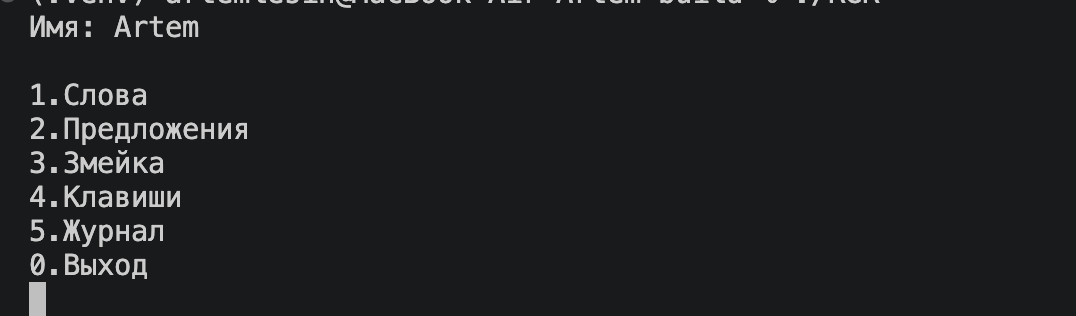
\includegraphics[width=0.8\textwidth]{photo/photo1.png}
    \caption{Главное меню программы}
\end{figure}

\begin{figure}[H]
    \centering
    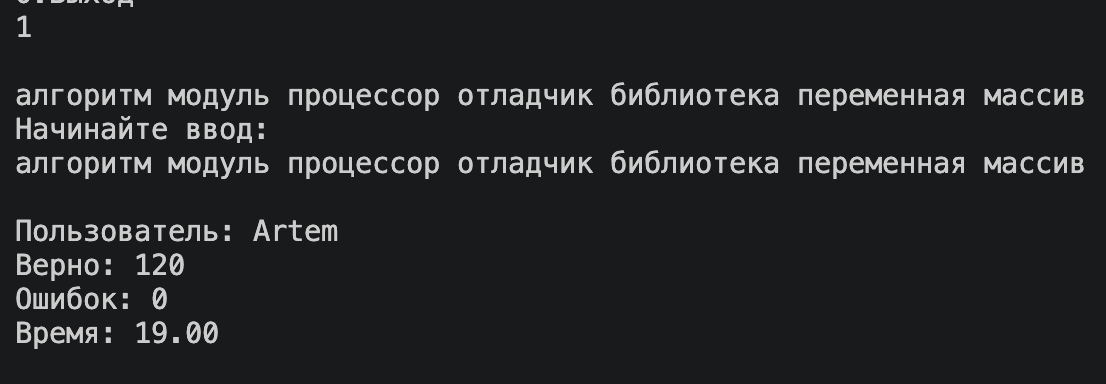
\includegraphics[width=0.8\textwidth]{photo/photo2.png}
    \caption{Режим тренировки слов}
\end{figure}

\begin{figure}[H]
    \centering
    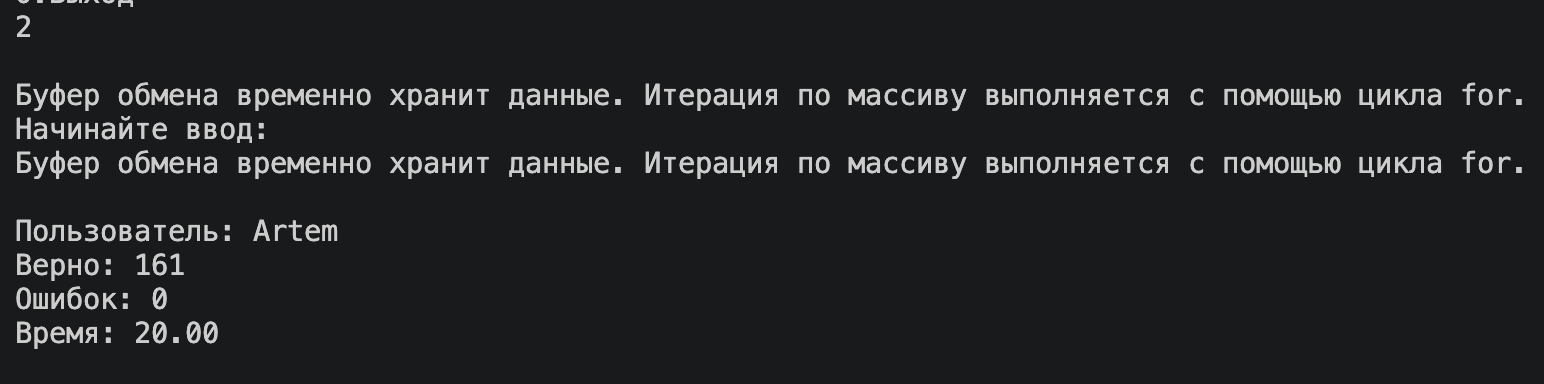
\includegraphics[width=0.8\textwidth]{photo/photo3.png}
    \caption{Режим предложений}
\end{figure}

\begin{figure}[H]
    \centering
    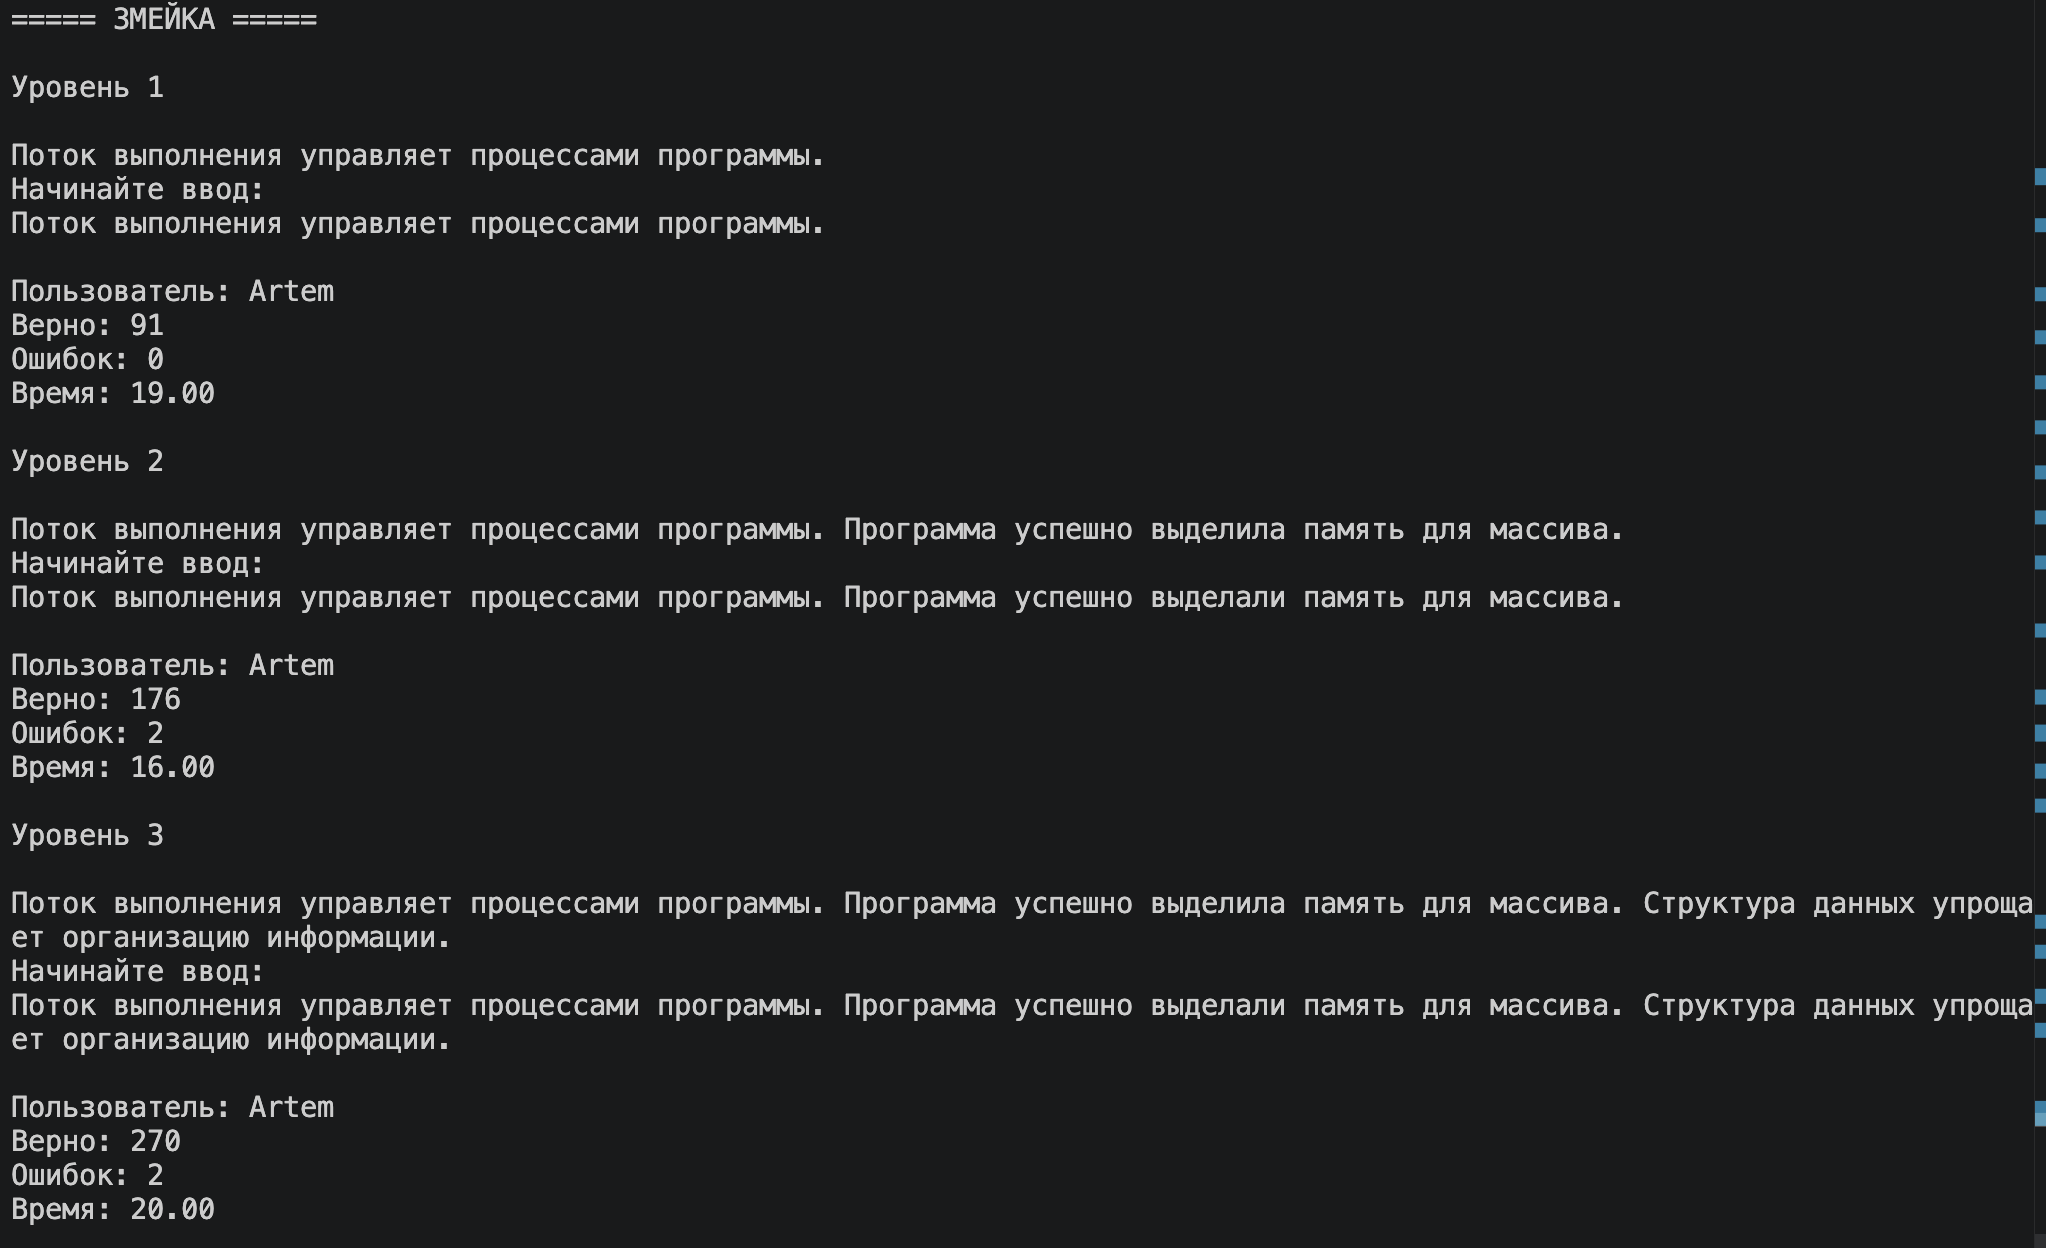
\includegraphics[width=0.8\textwidth]{photo/photo4.png}
    \caption{Режим «Змейка»}
\end{figure}

\begin{figure}[H]
    \centering
    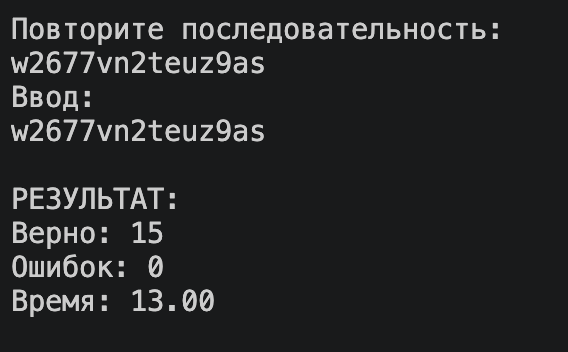
\includegraphics[width=0.8\textwidth]{photo/photo5.png}
    \caption{Режим тренировки клавиш}
\end{figure}

\begin{figure}[H]
    \centering
    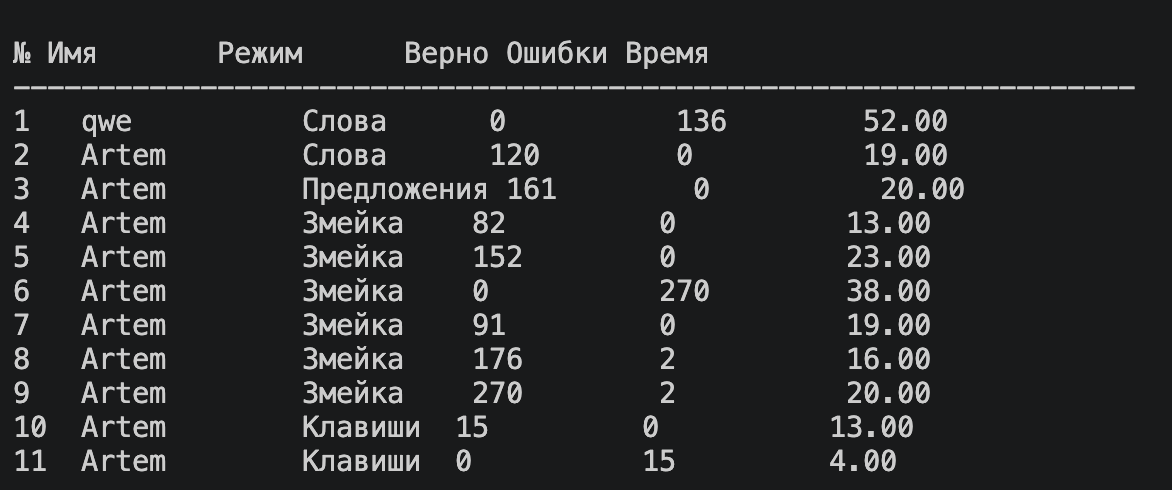
\includegraphics[width=0.8\textwidth]{photo/photo6.png}
    \caption{Журнал результатов}
\end{figure}

\begin{figure}[H]
    \centering
    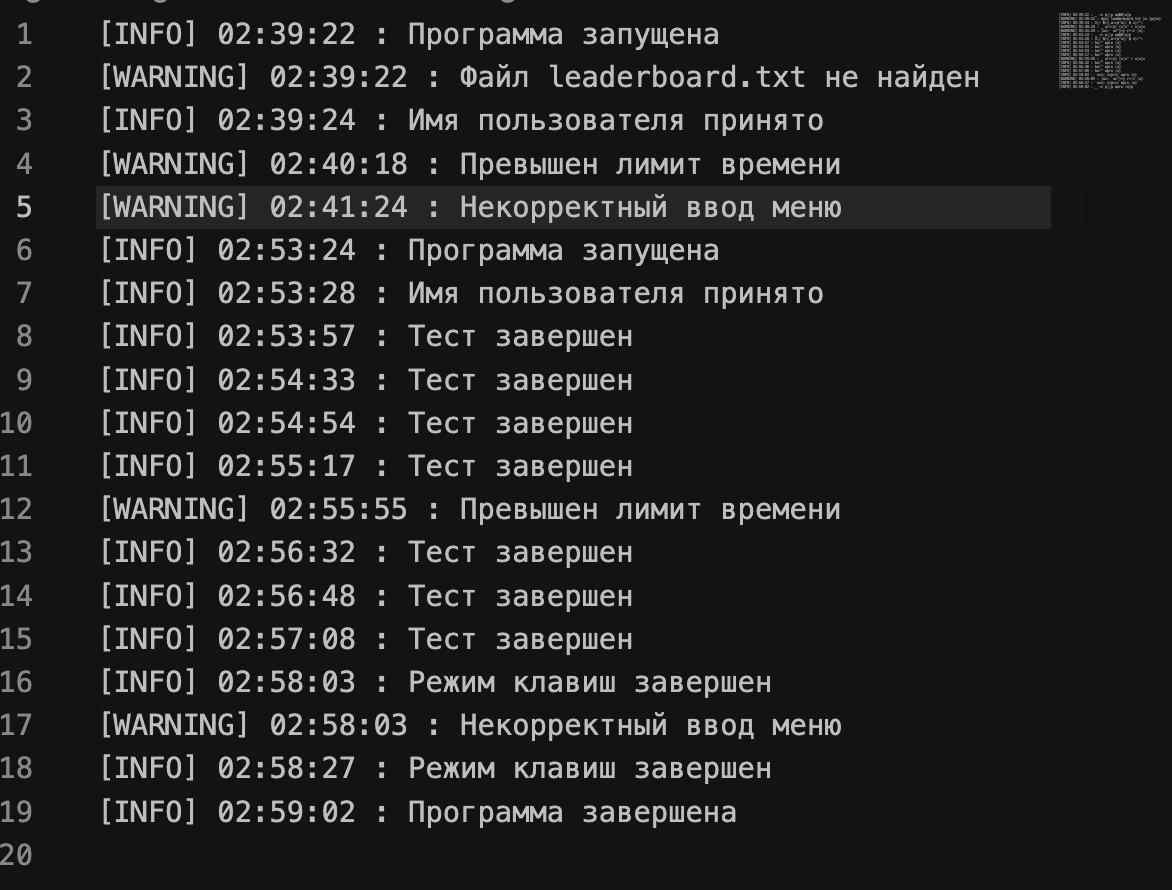
\includegraphics[width=0.8\textwidth]{photo/photo7.png}
    \caption{Пример логирования}
\end{figure}


\end{document}